\documentclass[11pt]{article}

\usepackage[margin=1in]{geometry}
\usepackage[T1]{fontenc}
\usepackage[utf8]{inputenc}
\usepackage{lmodern}
\usepackage{microtype}

\usepackage{xcolor}
\usepackage{graphicx}
\usepackage{array}
\usepackage{booktabs}
\usepackage{tabularx}
\usepackage{enumitem}
\usepackage{hyperref}
\usepackage{xurl}
\usepackage{amssymb}
\usepackage{qrcode}
\usepackage[most]{tcolorbox}
\usepackage{tikz}
\usetikzlibrary{calc,positioning,shapes.geometric}

\setlength{\parindent}{0pt}
\setlength{\parskip}{6pt}
\renewcommand{\arraystretch}{1.2}

\definecolor{BeeYellow}{HTML}{F4C430}
\definecolor{HiveBrown}{HTML}{B07A3F}
\definecolor{FlowerPink}{HTML}{D81B60}
\definecolor{PesticideRed}{HTML}{C62828}
\definecolor{SkyBlue}{HTML}{1976D2}

\tcbset{
  enhanced,
  sharp corners,
  boxrule=0.8pt,
  colback=white,
  colframe=black!40,
  left=10pt,
  right=10pt,
  top=8pt,
  bottom=8pt
}

\newtcolorbox{callout}[2][]{
  breakable,
  colback=black!2,
  colframe=black!35,
  title={#2},
  fonttitle=\bfseries,
  #1
}

\newcommand{\checkbox}{\(\square\)}

\newcommand{\BeeIcon}{%
  \tikz[baseline=-0.6ex,scale=0.23]{
    \draw[fill=BeeYellow,draw=black,line width=0.6pt] (0,0) ellipse (1.8 and 1.2);
    \draw[line width=0.6pt] (-0.9,0.8) .. controls (-1.6,1.6) and (-0.6,2.1) .. (0,1.4);
    \draw[line width=0.6pt] (0.9,0.8) .. controls (1.6,1.6) and (0.6,2.1) .. (0,1.4);
    \draw[line width=2.2pt] (-0.5,-1.0) -- (-0.5,1.0);
    \draw[line width=2.2pt] (0.2,-1.1) -- (0.2,1.1);
    \fill (1.55,0.25) circle (0.12);
  }%
}

\newcommand{\HiveIcon}{%
  \tikz[baseline=-0.6ex,scale=0.23]{
    \node[regular polygon,regular polygon sides=6,minimum size=9.5mm,draw=black,fill=HiveBrown!60] (h) {};
    \node[draw=black,fill=HiveBrown!20,rounded corners=1pt,minimum width=3.2mm,minimum height=2.2mm] at (h.center) {};
  }%
}

\newcommand{\FlowerIcon}{%
  \tikz[baseline=-0.6ex,scale=0.23]{
    \foreach \a in {0,60,120,180,240,300} {
      \draw[fill=FlowerPink!65,draw=black,line width=0.4pt] (\a:1.2) circle (0.7);
    }
    \draw[fill=BeeYellow!70,draw=black,line width=0.5pt] (0,0) circle (0.75);
  }%
}

\newcommand{\PesticideIcon}{%
  \tikz[baseline=-0.6ex,scale=0.23]{
    \node[regular polygon,regular polygon sides=3,minimum size=10mm,draw=black,fill=PesticideRed!55] (t) {};
    \node at ($(t.center)+(0,-0.5)$) {\bfseries\Large !};
  }%
}

\hypersetup{
  colorlinks=true,
  linkcolor=black,
  urlcolor=blue,
  citecolor=black
}

\newcolumntype{L}{>{\raggedright\arraybackslash}p{0.28\textwidth}}
\newcolumntype{R}{>{\raggedright\arraybackslash}X}

\title{Block Coding with Bees}
\author{}
\date{}

\begin{document}
\maketitle

\begin{callout}[colback=SkyBlue!4,colframe=SkyBlue!60!black]{Substitute Snapshot (Print this page)}
\begin{tabularx}{\textwidth}{@{}p{0.48\textwidth}X@{}}
\textbf{Goal} & Get the \BeeIcon{} bee from start to \HiveIcon{} hive while visiting all \FlowerIcon{} flowers and avoiding \PesticideIcon{} pesticide, using at least one loop.\\[4pt]
\textbf{Time} &
\begin{itemize}[leftmargin=*, itemsep=2pt, topsep=2pt]
  \item 10 min: Ignite Thinking (pictures + notice/wonder)
  \item 30--35 min: Work Time (review arrows \(\rightarrow\) block coding + loops)
  \item 10 min: Reflection (group process + debugging)
\end{itemize}
\\
\textbf{Board/Slide Directions} &
\begin{itemize}[leftmargin=*, itemsep=2pt, topsep=2pt]
  \item ``Use arrows first. Then convert to blocks and add a loop.''
  \item ``Run your program. If it fails, fix the bug and try again.''
\end{itemize}
\\
\textbf{Links (QR + click)} &
\begin{minipage}[t]{\linewidth}
\begin{tabular}{@{}p{0.70\linewidth}p{0.26\linewidth}@{}}
\href{https://docs.google.com/presentation/d/1G4IpqZIOp2TA8rVbL_0ee6OcGJEQgzUFjs5EIqG4TUI/edit?usp=drive_link}{Lesson slides} &
\qrcode[height=0.75in]{https://docs.google.com/presentation/d/1G4IpqZIOp2TA8rVbL_0ee6OcGJEQgzUFjs5EIqG4TUI/edit?usp=drive_link}
\\[2pt]
\href{https://drive.google.com/file/d/1ClL1QXeXpdP8ZqEM5PqSFkxkPQmzM-Ar/view?usp=drive_link}{Grid Image Cards} &
\qrcode[height=0.75in]{https://drive.google.com/file/d/1ClL1QXeXpdP8ZqEM5PqSFkxkPQmzM-Ar/view?usp=drive_link}
\\[2pt]
\href{https://drive.google.com/file/d/1CcwKTvvuaAUUFdJQmUwmJLqmrSo3At6b/view?usp=drive_link}{Coding Blocks} &
\qrcode[height=0.75in]{https://drive.google.com/file/d/1CcwKTvvuaAUUFdJQmUwmJLqmrSo3At6b/view?usp=drive_link}
\\
\end{tabular}
\end{minipage}
\\
\end{tabularx}
\end{callout}

\vspace{6pt}

\begin{callout}[colback=black!2,colframe=black!35]{Visual Legend (use while teaching)}
\begin{tabularx}{\textwidth}{@{}XXXX@{}}
\BeeIcon{} \textbf{Bee (student)} & \HiveIcon{} \textbf{Hive (goal)} & \FlowerIcon{} \textbf{Flower (must visit)} & \PesticideIcon{} \textbf{Pesticide (avoid)} \\
\end{tabularx}
\end{callout}

\section*{Lesson Overview}
\begin{tabularx}{\textwidth}{@{}LR@{}}
\toprule
\textbf{Pillar} & Computational Thinking \\
\textbf{Grade} & 2--3 \\
\textbf{Group Size} & 2--3 \\
\textbf{Essential Questions} &
\begin{itemize}[leftmargin=*, itemsep=2pt, topsep=2pt]
  \item How can loops and block coding be used to simplify an algorithm?
  \item What is block coding?
  \item How does block coding work?
  \item What is a loop?
\end{itemize}
\\
\textbf{Criteria for Success} & Code the bee to get it from its starting point to the beehive. Use block coding to communicate the bee's route to others. \\
\textbf{Constraints} &
\begin{itemize}[leftmargin=*, itemsep=2pt, topsep=2pt]
  \item The bee must pollinate all of the flowers.
  \item The bee must avoid the pesticide.
  \item Use at least 1 loop in your code.
\end{itemize}
\\
\bottomrule
\end{tabularx}

\section*{Learning Targets (Standards)}
\begin{itemize}[leftmargin=*, itemsep=2pt]
  \item I can decompose a problem into smaller steps, in multiple ways (2--3.CT.4).
  \item I can identify the essential information needed to get the Bee to the hive (2--3.CT.5).
  \item I can code using fixed and changing pieces of information (2--3.CT.7).
  \item I can document my plan to get the bee to the hive using block-coding (2--3.CT.10).
\end{itemize}

\section*{CASEL Competencies / SEL Standards}
\textbf{Habit 2: Begin with the End in Mind}
\begin{itemize}[leftmargin=*, itemsep=2pt, topsep=2pt]
  \item Set a short-term goal and begin working towards it (1c.2a).
  \item Identify steps in reaching the goal (1c.2b).
\end{itemize}

\textbf{Habit 5: Seek First to Understand, then Be Understood}
\begin{itemize}[leftmargin=*, itemsep=2pt, topsep=2pt]
  \item Identify verbal, physical, and situational cues that indicate how others may feel (2A.2a).
  \item Communicate perceived understanding of the expressed feelings and perspectives of others (2A.2b).
\end{itemize}

\section*{Materials}
\begin{itemize}[leftmargin=*, itemsep=2pt]
  \item Lesson slides: \href{https://docs.google.com/presentation/d/1G4IpqZIOp2TA8rVbL_0ee6OcGJEQgzUFjs5EIqG4TUI/edit?usp=drive_link}{Google Slides}
  \item Scissors
  \item Pencils
  \item 1 set per group of each of the following:
  \begin{itemize}[leftmargin=*, itemsep=2pt, topsep=2pt]
    \item Grid (large poster floor grid or painter's tape grid)
    \item Arrow cards from previous floor coding lessons
    \item Grid Image Cards: \href{https://drive.google.com/file/d/1ClL1QXeXpdP8ZqEM5PqSFkxkPQmzM-Ar/view?usp=drive_link}{Google Drive file}
    \item Coding Blocks: \href{https://drive.google.com/file/d/1CcwKTvvuaAUUFdJQmUwmJLqmrSo3At6b/view?usp=drive_link}{Google Drive file}
  \end{itemize}
\end{itemize}

\begin{callout}[colback=BeeYellow!10,colframe=BeeYellow!70!black]{Sub-Friendly Prep Checklist}
\begin{itemize}[leftmargin=*, itemsep=4pt, topsep=2pt]
  \item \checkbox{} Put up the floor grid (or tape grid) before students arrive.
  \item \checkbox{} Place Bee/Hive/Flower/Pesticide picture cards (or show the grid image on the board).
  \item \checkbox{} Give each group arrow cards and block-coding cards.
  \item \checkbox{} Decide a ``driver'' and ``checker'' role (swap halfway).
\end{itemize}
\end{callout}

\section*{Mini Visual: Example Grid (replace with your slide image)}
\begin{center}
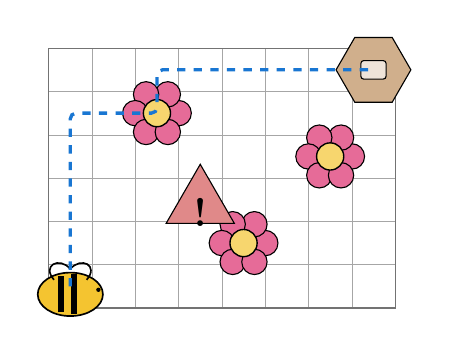
\begin{tikzpicture}[scale=0.55]
  % Grid
  \draw[step=1cm,black!35,very thin] (0,0) grid (8,6);
  \draw[black!55] (0,0) rectangle (8,6);

  % Legend items on grid
  \node at (0.5,0.5) {\BeeIcon{}};
  \node at (7.5,5.5) {\HiveIcon{}};
  \node at (2.5,4.5) {\FlowerIcon{}};
  \node at (4.5,1.5) {\FlowerIcon{}};
  \node at (6.5,3.5) {\FlowerIcon{}};
  \node at (3.5,2.5) {\PesticideIcon{}};

  % Light suggested path (dashed) for explanation only
  \draw[SkyBlue,very thick,dashed,rounded corners=2pt]
    (0.5,0.5) -- (0.5,4.5) -- (2.5,4.5) -- (2.5,5.5) -- (7.5,5.5);
\end{tikzpicture}
\end{center}
\textit{Tip: Use this diagram only as a teaching aid. Students should match the official grid image from the slides/smartboard.}

\section*{Lesson Structure}
\begin{tabularx}{\textwidth}{@{}L R@{}}
\toprule
\textbf{Phase (Time)} & \textbf{Plan} \\
\midrule
\textbf{Ignite Thinking (10 mins)} &
\begin{minipage}[t]{\linewidth}
\begin{itemize}[leftmargin=*, itemsep=2pt, topsep=2pt]
  \item Show students images of bees:
  \begin{itemize}[leftmargin=*, itemsep=2pt, topsep=2pt]
    \item Image 1: Bee pollinating a flower
    \item Image 2: Danger of pesticides
  \end{itemize}
  \item Ask students what they notice and know about these pictures.
  \item Tell students they will use coding knowledge to help bees navigate through an ecosystem full of flowers and pesticides.
  \item Review learning targets.
\end{itemize}
\end{minipage}
\\
\textbf{Work Time (30--35 mins)} &
\begin{minipage}[t]{\linewidth}
\begin{enumerate}[leftmargin=*, itemsep=4pt, topsep=2pt]
  \item \textbf{Task 1: Arrow Coding Review} (\textasciitilde{}5--7 minutes)\\
  Have students set up their floor grids to match the image on the smartboard. Students work in their groups using arrow cards to get the bee to the hive (keeping constraints in mind).
  \item \textbf{Introduce Block Coding} (\textasciitilde{}5 minutes)\\
  Introduce block coding and describe what it is. Ask how often they had a step/arrow repeat; introduce the vocabulary term \emph{loop}. Review essential questions and vocabulary terms.
  \item \textbf{Task 2: Turn Arrow Coding into Block Coding} (\textasciitilde{}5 minutes)\\
  Whole-group: Model changing arrow codes into blocks with loops. Introduce \textbf{Run} and \textbf{End} commands.
  \item \textbf{Task 3: Block Coding} (\textasciitilde{}15--20 minutes)\\
  Students set up their floor grids to match the image on the smartboard. Students work in their groups using block coding to get the bee to the hive. If time, have groups switch places and run each other's program to see if it works or if there are bugs.
\end{enumerate}
\end{minipage}
\\
\textbf{Reflection (10 mins)} &
\begin{minipage}[t]{\linewidth}
Use look-fors/documentation during discussion:
\begin{itemize}[leftmargin=*, itemsep=2pt, topsep=2pt]
  \item How did you feel about block coding?
  \item What went well in your group?
  \item How did you make sure that everyone's perspectives were heard in your group?
  \item Anything from the look-fors?
\end{itemize}
\end{minipage}
\\
\bottomrule
\end{tabularx}

\section*{Look Fors / Document}
\begin{itemize}[leftmargin=*, itemsep=2pt]
  \item Students using talking points, actively listening to each other, and taking turns/hearing other perspectives.
  \item Groups that handle conflict well.
  \item Examples of programs using block coding accurately or with bugs that need to be fixed.
\end{itemize}

\begin{callout}[colback=black!2,colframe=black!35]{Common Sticking Points (quick fixes)}
\begin{itemize}[leftmargin=*, itemsep=4pt, topsep=2pt]
  \item \textbf{Missed a flower:} Have students highlight/check off each \FlowerIcon{} flower as they ``visit'' it.
  \item \textbf{Hit pesticide:} Ask, ``Which step took you onto \PesticideIcon{}?'' Remove or change that step.
  \item \textbf{Loop confusion:} Identify the repeating pattern first, then wrap it in a loop (e.g., repeat 3 times).
  \item \textbf{Group conflict:} Use roles (driver/checker) and a 30-second ``listen first'' turn.
\end{itemize}
\end{callout}

\end{document}
